\section{Base model construction}
\subsection{Platform for infectious disease dynamics simulation}

We developed a deterministic compartmental model of COVID-19 transmission using the AuTuMN platform,
publicly available at https://github.com/monash-emu/AuTuMN/.
Our repository allows for the rapid and robust creation and stratification of models of infectious disease epidemiology
and includes pluggable modules to simulate heterogeneous population mixing, demographic processes, multiple circulating
pathogen strains, repeated stratification and other dynamics relevant to infectious disease transmission.
The platform was created to simulate TB dynamics, being an infectious disease whose epidemiology differs markedly
by setting, such that considerable flexibility is desirable \cite{RN58}.
We have progressively developed the structures of our platform over recent years,
and further adapted it to be sufficiently flexible
to permit simulation of other infectious diseases for the purpose of this project.

\subsection{Base COVID-19 model}
Using the base framework of an SEIR model (susceptible, exposed, infectious, removed), we split the exposed and infectious compartments into two sequential compartments each (SEEIIR). The two sequential exposed compartments represent the non-infectious and infectious phases of the incubation period, with the latter representing the ``presymptomatic" phase such that infectiousness occurs during three of the six sequential phases. For this reason, ``active" is a more accurate term for the two sequential ``I" compartments and is preferred henceforward. The two infectious compartments represent early and late phases of active disease, during which symptoms occur if the disease episode is symptomatic, and allow explicit representation of notification, case isolation, hospitalisation and admission to ICU. The ``active" compartment also includes some persons who remain asymptomatic throughout their disease episode, such that these compartments do not map directly to either persons who are infectious or those who are symptomatic.


\begin{figure}[ht!]
    \centering
    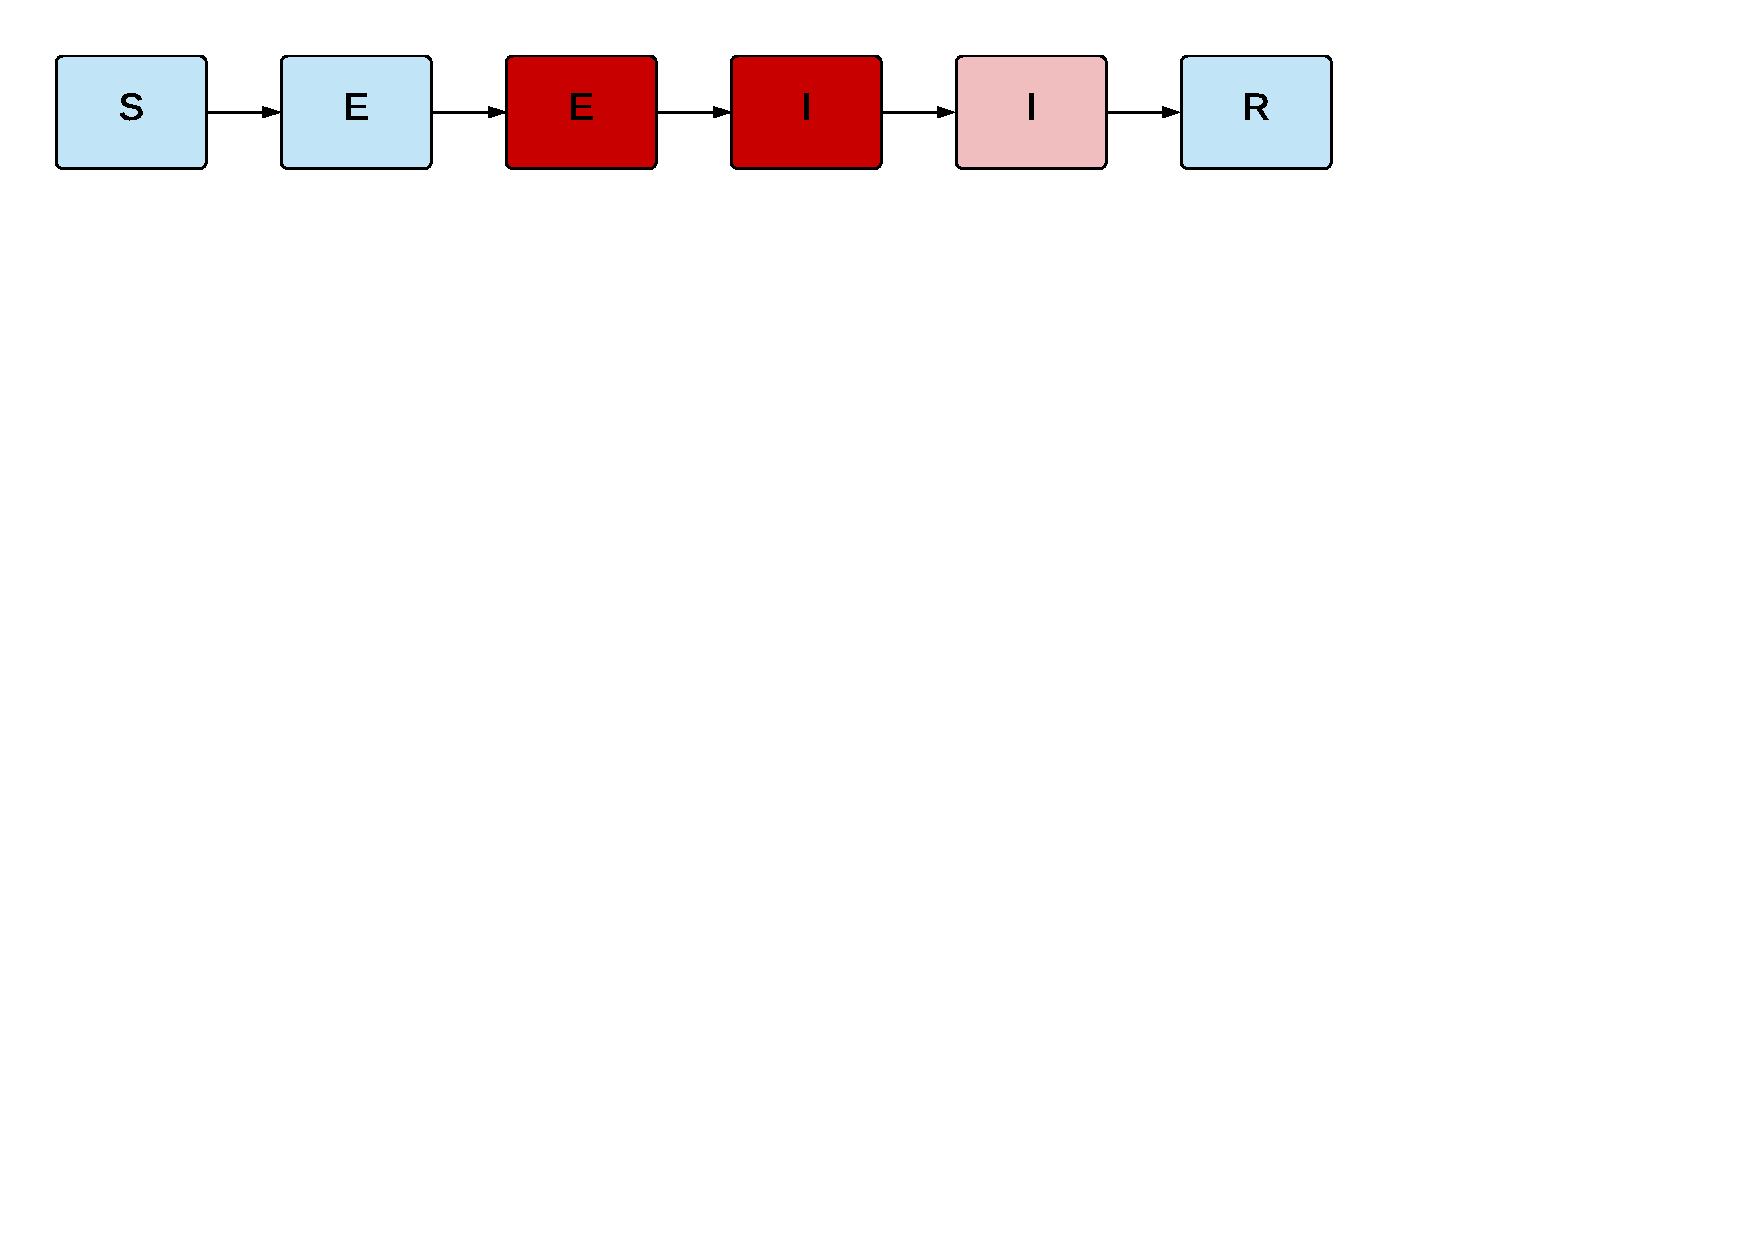
\includepdf{../model/covid_19_seeiir.pdf}
    \caption{\textbf{Unstratified compartmental model structure.} S = susceptible, E = exposed, I = active, R = recovered/removed. Depth of pink/red shading indicates the infectiousness of the compartment.}
    \label{fig:seeiir}
\end{figure}
